\documentclass[10pt,a4paper]{article}
\usepackage[T1]{fontenc}
\usepackage[utf8]{inputenc}
\usepackage{lmodern,microtype}
\usepackage[margin=22mm,headheight=14pt]{geometry}
\usepackage{graphicx,booktabs,longtable,array,ragged2e}
\usepackage{fvextra}
\usepackage{float}
\usepackage{xcolor}
\usepackage{caption,subcaption}
\usepackage{amsmath,amssymb}
\usepackage{seqsplit}
\usepackage{fancyhdr}
\usepackage{tikz}
\usetikzlibrary{arrows.meta}
\usepackage[hidelinks]{hyperref}
\usepackage{url}
\definecolor{navy}{HTML}{24547A}
\hypersetup{colorlinks=true,linkcolor=navy,urlcolor=navy,citecolor=navy}
\urlstyle{tt}
\setlength{\parskip}{4pt}
\setlength{\parindent}{0pt}
\captionsetup{font=small,labelfont=bf}
\pagestyle{fancy}
\fancyhf{}
\fancyhead[L]{\small NumStability benchmark | ten-task evidence report}
\fancyhead[R]{\small 28 September 2026}
\fancyfoot[C]{\thepage}
\newcommand{\src}[1]{\textsuperscript{\cite{#1}}}
\newcommand{\fig}[2]{%
\begin{figure}[p]\centering
\includegraphics[width=.96\textwidth]{../benchmark/figures/#1.pdf}
\caption{#2 All task values are derived from the sealed N/L pairs by the
reproducible ten-task plotting script.\cite{taskledger,plotcode}}
\end{figure}}
\newcommand{\phaseoutfig}[2]{%
\begin{figure}[p]\centering
\includegraphics[width=.96\textwidth]{../benchmark/figures/#1.pdf}
\caption{#2 Values are calculated from the sealed paired ledger by the
phase-outcome plotting script.\cite{taskledger,phaseplotcode}}
\end{figure}}
\newcommand{\metricfig}[3]{%
\begin{figure}[H]\centering
\begin{tikzpicture}
\node[inner sep=0] (plot) {\includegraphics[width=.96\textwidth]{../benchmark/figures/#1.pdf}};
\node[anchor=north west,xshift=1.8cm,yshift=-.35cm,
      fill=white,fill opacity=.93,text opacity=1,draw=black!25,
      rounded corners=2pt,inner sep=3pt,font=\footnotesize]
      at (plot.north west) {Spearman $\rho=#3$ ($n=10$)};
\end{tikzpicture}
\caption{#2 Exact coordinates are derived from the sealed paired ledger;
numbered points match Table~\ref{tab:usecounts}. The displayed Spearman
coefficient uses unrounded gains and average ranks for any ties; it is
descriptive, not causal.\cite{phasepoints,usagepoints,metriccode}}
\end{figure}}
\newcommand{\usagefig}[2]{%
\begin{figure}[H]\centering
\includegraphics[width=\textwidth]{../benchmark/figures/#1.pdf}
\caption{#2 Each numbered point identifies a task in
Table~\ref{tab:usecounts}; the three panels give total active-time,
kernel-accepted proof-line, and net-new-token gains. Each panel prints its
Spearman rank coefficient for all ten tasks. These are descriptive,
post-run associations, not causal estimates.\cite{usagepoints,metriccode,taskledger}}
\end{figure}}
\newcommand{\suppfig}[2]{%
\begin{figure}[H]\centering
\includegraphics[width=\textwidth]{../benchmark/figures/#1.pdf}
\caption{#2 Numbered points match Table~\ref{tab:suppcounts}. Positive
percentage gains favor L. These secondary diagnostics are not measures of
direct proof reuse.\cite{usagepoints,metriccode}}
\end{figure}}
\newcommand{\phasefig}[2]{%
\begin{figure}[H]\centering
\includegraphics[width=\textwidth]{../benchmark/figures/#1.pdf}
\caption{#2 Numbered points identify tasks in
Table~\ref{tab:usecounts}. Positive percentage gains favor L; each panel
prints the Spearman coefficient across all ten tasks. These are
descriptive post-run associations, not causal estimates.\cite{phasepoints,metriccode}}
\end{figure}}
\title{\vspace{-13mm}\textbf{NumStability in AI-Assisted Lean Formalization and Proof}\\[2mm]
\large A reproducible, exploratory ten-task N/L benchmark report}
\author{HighamBench evidence report}
\date{28 September 2026}
\begin{document}
\maketitle

\begin{abstract}
We compare a Mathlib-only condition (N) with the same Lean environment plus a
frozen NumStability library and one task-neutral orientation conversation (L).
All ten paper tasks ended with an audited faithful statement and a
zero-hole, kernel-accepted proof in both conditions. Across these pairs, L
used 19.7\% fewer nonblank proof-code lines (2,537 versus 3,158) and 22.5\%
less contestant-active time (5,410 versus 6,979 seconds), while using 34.7\%
more net-new tokens (1.716 versus 1.273 million). Charging the one-time L
scout once leaves a 19.9\% time advantage and 41.7\% token excess. The
formalization stage was 7.3\% slower for L; the proof stage was 29.9\% faster.
The phase-matched direct-use counts have Spearman rank correlations of
$-0.12$ for statement use versus formalization-time gain, $+0.56$ for
proof use versus proof-time gain, and $+0.56$ for combined use versus
total-time gain. Other usage counts give different correlations.
Literal source-name counts are excluded because they miss namespace-open uses. These
are descriptive results from one run per task, not a causal estimate.
\src{summary,taskledger,usagepoints}
\end{abstract}

\section{Question and corpus}

The question is whether a numerical-stability library reduces the work and
Lean code needed for an AI formalizer to state \emph{and prove} selected paper
results. Both conditions receive the same hashed source paper, task packet,
Lean 4, Mathlib, formalization prompt, audit policy, and proof requirement. L
alone receives frozen NumStability source and compiled declarations plus an
orientation appendix.

The ten analyzed tasks span five source clusters: three Castaldo--Whaley--
Chronopoulos dot-product tasks, four Blanchard--Higham--Higham
log-sum-exp/softmax tasks, and one each from Hallman--Ipsen, Higham, and Rump.
Four tasks were marked hard in the frozen task metadata.
\src{summary,registry,taskledger}

The measured result combines sealed pairs from two campaign identities.
The private pair archives retain prompts, candidate hashes, audit decisions,
accepted Lean files, proof checks, and hardware records. Pair reports
preserve source SHA-256 values and condition order.
\src{taskledger,evidence}

\begin{table}[ht]\centering\small
\begin{tabular}{@{}llrl@{}}\toprule
Cluster & Source & Tasks & PDF SHA-256 prefix\\\midrule
CAST08 & Castaldo et al., superblock dot product & 3 & \texttt{ffdea8e2136c7f42}\\
H20 & Higham, \emph{Accuracy and Stability}, Problem 20.8 & 1 & \texttt{7ca85d5caf3ffd5a}\\
HI21 & Hallman--Ipsen, summation-tree bounds & 1 & \texttt{cce25923a86d5d20}\\
P14 & Blanchard et al., log-sum-exp/softmax & 4 & \texttt{7247047bc49218e0}\\
RUMP12 & Rump, summation/dot-product error & 1 & \texttt{4b23ffc2f7588ddc}\\
\bottomrule\end{tabular}
\caption{Five paper/source clusters. Task-packet and paper-PDF hashes are
in \texttt{benchmark/results/source\_registry.json}.\cite{registry,packets}}
\label{tab:papers}
\end{table}

\section{Protocol and archived execution}

\subsection{Two stages, two clocks, and an independent audit}

A contestant first submits a Lean theorem with a single allowed
\texttt{sorry} occupying its target proof. There are at most four frozen
statement submissions. Each is hashed before off-clock compilation,
integrity validation, and independent candidate-specific faithfulness audit.
An unfaithful statement receives condition-neutral feedback in the same
formalizer conversation. Once a faithful statement is frozen, the model gets
up to four submissions to prove that \emph{exact proposition}. A proof with
\texttt{sorry}, \texttt{admit}, changed dependencies, extra axioms, or a trust
escape is not accepted. Proof success requires zero-hole Lean validation.
The formalizer is explicitly told not to submit a partial proof as complete.
\src{protocol,prompts,taskledger}

\begin{figure}[ht]\centering
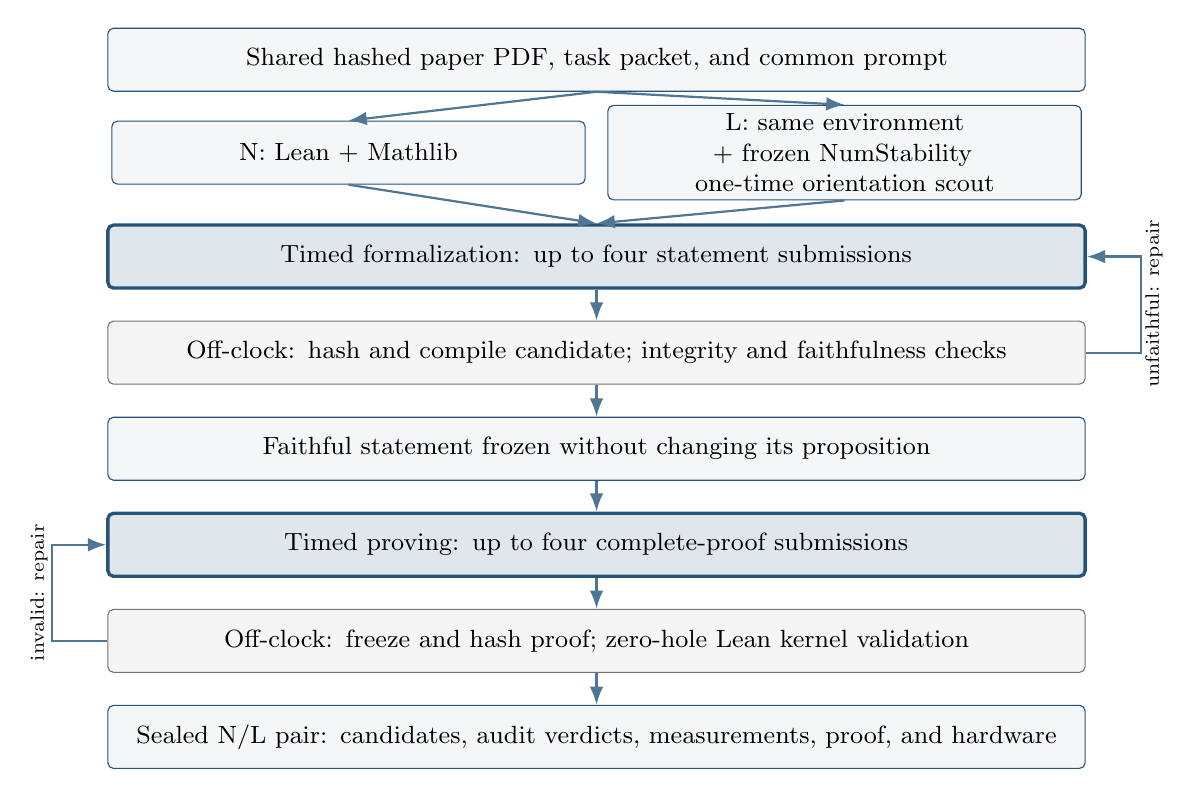
\begin{tikzpicture}[
  >=Latex,
  box/.style={draw=navy, rounded corners=2pt, align=center,
    minimum height=8mm, inner sep=3pt, font=\small},
  shared/.style={box, fill=navy!5},
  active/.style={box, fill=navy!14, very thick},
  check/.style={box, draw=black!55, fill=black!4},
  arr/.style={->, thick, draw=navy!80}
]
\node[shared, text width=12.2cm] (source) at (0,0)
  {Shared hashed paper PDF, task packet, and common prompt};
\node[shared, text width=5.8cm] (n) at (-3.15,-1.18)
  {N: Lean + Mathlib};
\node[shared, text width=5.8cm] (l) at (3.15,-1.18)
  {L: same environment + frozen NumStability\\one-time orientation scout};
\node[active, text width=12.2cm] (statement) at (0,-2.50)
  {Timed formalization: up to four statement submissions};
\node[check, text width=12.2cm] (audit) at (0,-3.72)
  {Off-clock: hash and compile candidate; integrity and faithfulness checks};
\node[shared, text width=12.2cm] (frozen) at (0,-4.94)
  {Faithful statement frozen without changing its proposition};
\node[active, text width=12.2cm] (proof) at (0,-6.16)
  {Timed proving: up to four complete-proof submissions};
\node[check, text width=12.2cm] (kernel) at (0,-7.38)
  {Off-clock: freeze and hash proof; zero-hole Lean kernel validation};
\node[shared, text width=12.2cm] (record) at (0,-8.60)
  {Sealed N/L pair: candidates, audit verdicts, measurements, proof, and hardware};
\draw[arr] (source.south) -- (n.north);
\draw[arr] (source.south) -- (l.north);
\draw[arr] (n.south) -- (statement.north);
\draw[arr] (l.south) -- (statement.north);
\draw[arr] (statement.south) -- (audit.north);
\draw[arr] (audit.south) -- (frozen.north);
\draw[arr] (frozen.south) -- (proof.north);
\draw[arr] (proof.south) -- (kernel.north);
\draw[arr] (kernel.south) -- (record.north);
\draw[arr] (audit.east) -- ++(.70,0) |- (statement.east);
\draw[arr] (kernel.west) -- ++(-.70,0) |- (proof.west);
\node[font=\scriptsize, fill=white, inner sep=1pt, rotate=90]
  at (7.08,-3.10) {unfaithful: repair};
\node[font=\scriptsize, fill=white, inner sep=1pt, rotate=90]
  at (-7.08,-6.77) {invalid: repair};
\end{tikzpicture}
\caption{Source-first workflow. Blue boxes are contestant-active and timed;
gray boxes are independently checked off-clock. Failed checks return
condition-neutral feedback within the same stage. Auditing and validation
are excluded from contestant-active clocks.\cite{protocol,metrics}}
\label{fig:flow}
\end{figure}

Faithfulness is binary. A full-domain equivalent statement or accepted
strengthening may pass; a narrowing of the paper's domain does not. The audit
uses fresh, stateless and condition-blind blind-translation, direct,
round-trip, and adjudication roles with dependency-aware semantic material.
These agents are independent of the formalizers. A faithful statement is not
counted as a proof; the zero-hole proof gate is separate. Some accepted
statements are equivalent while others are strengthenings, which can affect
the proof effort even when both pass.\src{protocol,evidence,taskledger}

For every distinct candidate, the controller constructs a pseudonymized
semantic dossier from the elaborated target type and the definitions it
depends on; the target proof is excluded. A blind translator receives that
dossier without the source paper and translates the proposition and every
listed dependency into mathematical language. Independently, a direct judge
compares the dossier with the selected paper result. A round-trip judge then
compares the blind translation with the paper without seeing Lean, the
dossier, or the direct judgment. The paper PDF takes precedence over the
task packet if they disagree.\src{protocol,evidence}

Both judges account for each supplied dependency, complete the same 16
semantic checks (including binders, hypotheses, algorithm and norm meaning,
rounding model, domain, and nonvacuity), and judge each implication direction
separately. Genuine strengthening is accepted, but extra assumptions,
restricted or merely partial case coverage, and vacuous statements are not.
An unresolved check or disagreement goes to an independent adjudicator;
uncertainty is never silently accepted. A failed candidate receives only a
condition-neutral description of the missing paper requirement and candidate
mismatch, not a replacement Lean theorem, proof, or NumStability declaration
name. The candidate hash, role outputs, decision, and feedback are retained
in the pair archive.\src{protocol,evidence}

The formalizer was GPT-6 Sol at high reasoning effort in both conditions;
GPT-6 Astra/high performed auditing. Contestant subagents and multi-agent
tools were disabled and attested by session controls. Observable tool and
turn events were archived; hidden chain-of-thought was not available.
Access used ChatGPT sign-in through Codex CLI 0.156.0, not metered API
billing.\src{metrics,evidence,runtimesnapshot}

\subsection{Prompts and library access}

The common prompt says the PDF is authoritative and asks for the paper's
full domain, quantifiers, operation order, rounding model, constants, and
conclusion. It warns of independent faithfulness review and later proof.
N receives this prompt with Mathlib. L receives the same prompt plus a short
appendix encouraging deliberate discovery of the relevant algorithm
representation, compatible floating-point model, and error/perturbation
lemmas. L has access to the full library, not an oracle or task-specific
retrieval packet. A separate strict no-hole proof prompt is frozen. The
verbatim text of all five frozen task-neutral prompts appears in
Appendix~\ref{app:prompts}; the per-task source packet and effective
messages are retained in the run archives.\src{prompts,proofprompt,evidence}

\begin{table}[ht]\centering\small
\begin{tabular}{@{}ll@{}}\toprule
Prompt & SHA-256 prefix\\\midrule
Common statement & \texttt{c3ece6ddddf2b2c}\\
L treatment appendix & \texttt{579a68943cfb636}\\
Task-neutral scout & \texttt{f2517b44f0801c0}\\
Proof-stage base & \texttt{b21295790a3ff3f}\\
Strict no-hole proof prompt & \texttt{537ebad7810ec9a}\\
Audit roles & exact hashes in archived campaign inputs\\
\bottomrule\end{tabular}
\caption{Prompt identity; source files and observed effective prompts in the
archives provide full text.\cite{prompts,proofprompt,evidence}}
\end{table}

The task-neutral L scout ran once for 183.313 seconds using GPT-6 Sol/high.
It used 1,274,811 input tokens, 1,193,216 of them cached, plus 6,873 output
tokens: 88,468 net-new tokens by the benchmark formula. The provider total
including cached input was 1,281,684 tokens. Its frozen orientation root
was forked into task conversations; the scout was never rerun per task.
\src{warmroot,warmscout}

\subsection{Hardware, parallelism, and software}

Titan ran Linux/x86-64 on an Intel Core i9-13900K. Three disjoint lanes ran
concurrently, each capped at eight logical CPUs, 24~GiB RAM, zero swap, and
512 processes. N/L order alternated by frozen schedule index. CPU affinity,
cgroups, before/after machine snapshots, and sampled per-turn peaks were
logged. Across the ten tasks, sampled per-condition maxima were 5.39
cores and 2.35~GiB for N, and 4.70 cores and 2.01~GiB for L. Brief spikes
could be missed. Parallelism reduced campaign makespan; it did not divide
individual contestant-active time.\src{summary,evidence}

\begin{figure}[htbp]\centering
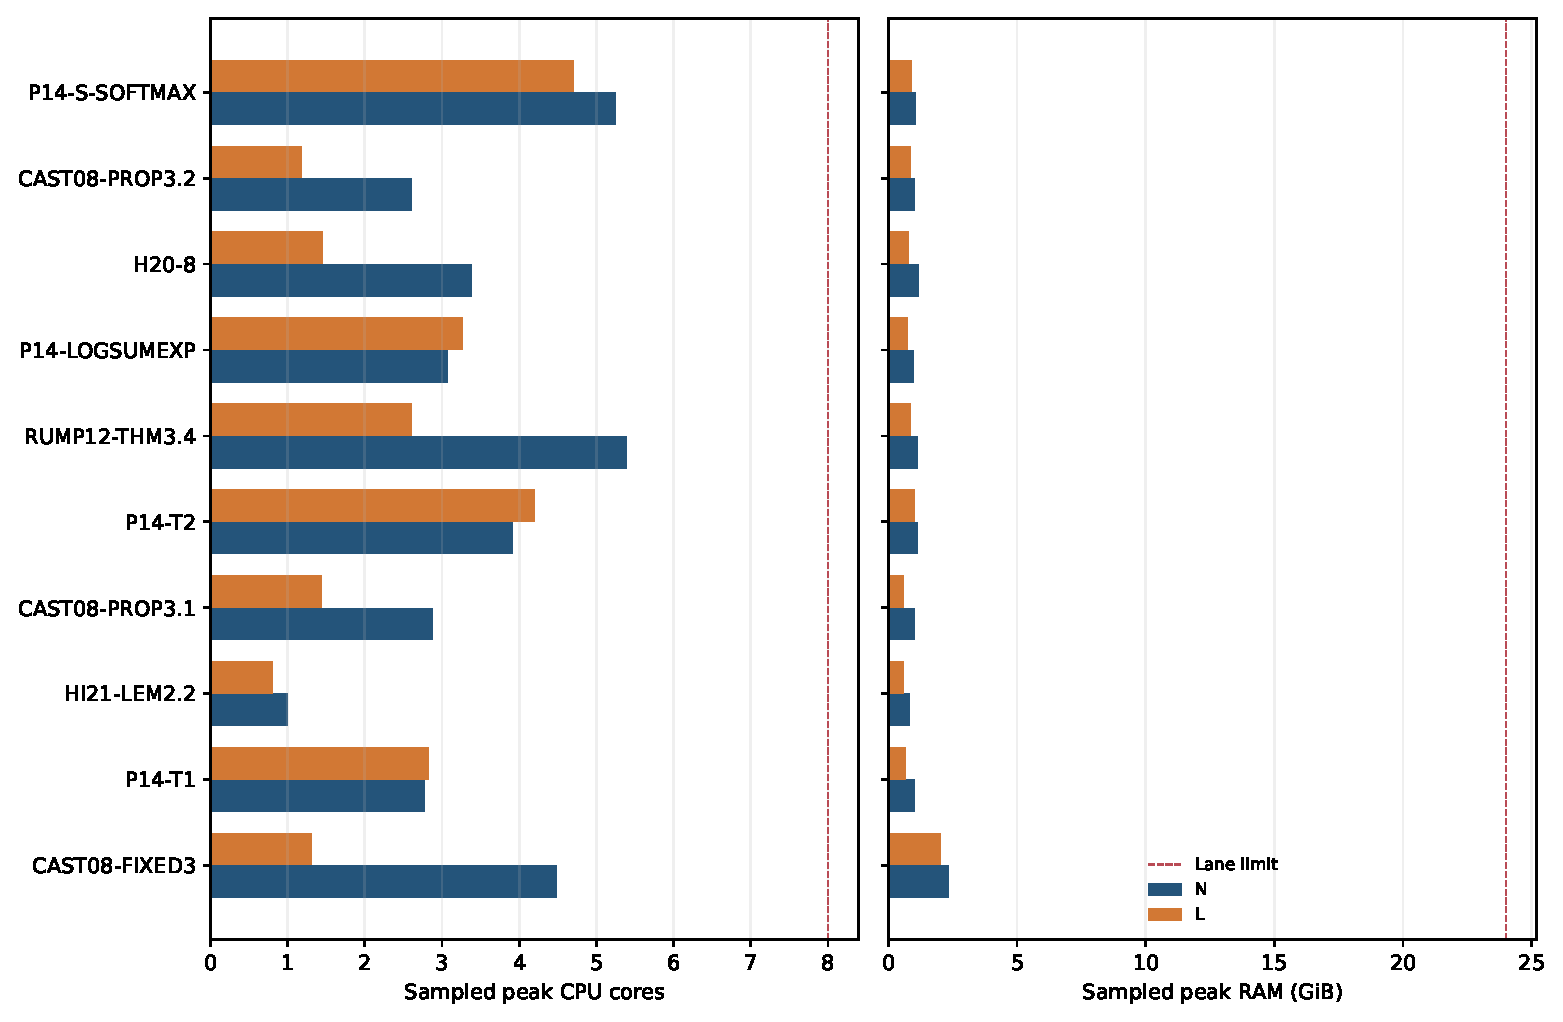
\includegraphics[width=.92\textwidth]{../benchmark/figures/13_hardware_peaks.pdf}
\caption{Sampled per-task CPU and RAM peaks against lane caps; brief
unobserved spikes are possible. Task labels identify the archived targets.
\cite{summary,taskledger}}
\end{figure}

Lean was \texttt{leanprover/lean4:v4.29.0-rc3}, Mathlib commit
\texttt{\seqsplit{e8ea1afc32790ce1d4e1a4e45cc412ba9388716b}}, and
NumStability commit
\texttt{\seqsplit{45813a95dacf577461bae13f033af0dbc985a225}}.
The separately recorded full-library build took 1,315.18 seconds after
Mathlib dependency-cache preparation; it is not charged to task-active time.
The build record identifies hardware, cache state, command, output digest,
and resource measurements. Authentication material and compiled caches are
not redistributed.\src{buildrecord,librarysnapshot,runtimesnapshot}

\section{Metrics and denominators}

Formalization time includes contestant-active work through the frozen
faithful statement, including ordinary library search and repairs. Proof
time starts after that statement is frozen and includes proof turns and
rejected submissions. Their sum is task-active time. Compilation, dossier
construction, and auditing are off-clock and excluded. The
headline time is neither whole campaign makespan nor end-to-end wall time.
Net-new tokens equal input minus cached input plus output; full provider
usage including cached input is retained separately. Code lines exclude
blank and comment-only lines. All ten pairs have faithful statements and
complete proofs in both conditions, so paired proof denominators are ten.
Warm-inclusive per-task panels allocate the one-time L scout evenly over ten
for visualization; aggregate and cumulative calculations charge it once.
Positive N-to-L gain means less L cost.\src{metrics,taskledger,warmroot}

\begin{table}[H]\centering\small
\begin{tabular}{@{}lrrrr@{}}\toprule
Metric (ten tasks, summed) & N & L & L/N & L gain on sums\\\midrule
Formalization seconds & 1,389.1 & 1,490.2 & 1.073 & -7.3\% \\
Proof seconds & 5,589.8 & 3,920.0 & 0.701 & +29.9\% \\
Total active seconds & 6,978.9 & 5,410.2 & 0.775 & +22.5\% \\
Total + warm seconds & 6,978.9 & 5,593.5 & 0.801 & +19.9\% \\
Formalization net-new tokens & 399,748 & 980,733 & 2.453 & -145.3\% \\
Proof net-new tokens & 873,571 & 734,899 & 0.841 & +15.9\% \\
Total net-new tokens & 1,273,319 & 1,715,632 & 1.347 & -34.7\% \\
Total + warm net-new tokens & 1,273,319 & 1,804,100 & 1.417 & -41.7\% \\
Statement code lines & 333 & 337 & 1.012 & -1.2\% \\
Proof code lines & 3,158 & 2,537 & 0.803 & +19.7\% \\
\bottomrule

\end{tabular}
\medskip

\textit{Running cumulative L gain (\%) at scheduled checkpoints:}
\begin{tabular}{@{}lrrrr@{}}\toprule
Through task & Formal time & Proof time & Total time & Total + scout\\\midrule
1 & +8.6\% & +42.9\% & +35.9\% & +5.6\% \\
5 & -7.1\% & +34.5\% & +24.3\% & +17.9\% \\
10 & -7.3\% & +29.9\% & +22.5\% & +19.9\% \\
\bottomrule

\end{tabular}

\medskip

\begin{tabular}{@{}lrrrr@{}}\toprule
Through task & Formal tokens & Proof tokens & Total tokens & Total + scout\\\midrule
1 & -171.9\% & -98.4\% & -122.7\% & -202.7\% \\
5 & -176.4\% & +8.8\% & -58.4\% & -75.8\% \\
10 & -145.3\% & +15.9\% & -34.7\% & -41.7\% \\
\bottomrule

\end{tabular}
\caption{Ten-task sums (upper panel) and running cumulative percentage gains
after task 1, task 5, and task 10. At checkpoint $k$, gain is
$100(\sum_{i\leq k}N_i-\sum_{i\leq k}L_i)/\sum_{i\leq k}N_i$;
positive values favor L. ``+ scout'' adds the one-time L orientation cost
once, not once per task. The final checkpoint agrees with the ten-task
aggregate rows above.\cite{summary,taskledger,plotcode,phaseplotcode}}
\label{tab:aggregate}
\end{table}

\section{Time, token, and code outcomes}

L was faster on eight of ten tasks and used fewer proof-code lines on six of
ten. Formalization cost 7.3\% more active time and 2.45 times as many net-new
tokens for L; proof used 29.9\% less time and 15.9\% fewer net-new tokens.
Mean time was 697.9 seconds/task for N and 541.0 for L, or 559.3 with the
scout allocated. Mean net-new tokens were 127.3 thousand for N and 171.6
thousand for L, or 180.4 thousand with the scout. The time and proof-line
gains do not imply token savings. General outcome figures label tasks by
their archived IDs; the primary usage--gain figures below apply one
direct-declaration measure to three phase-matched surfaces instead of a
composite score.\src{summary,usagepoints,plotcode}

\fig{01_total_time_ex_warm}{Per-task total contestant-active time, excluding the one-time scout. Task-time library search remains included.}
\fig{02_total_time_in_warm}{Per-task active time with $183.313/10=18.331$ warm seconds allocated to each L bar. This is one scout, not ten.}
\phaseoutfig{03a_formalization_time}{Per-task formalization time through the audited faithful statement; task-time search and repairs are included.}
\phaseoutfig{03b_proof_time}{Per-task proof time after the faithful statement was frozen; rejected proof submissions are included.}
\fig{04_total_tokens_ex_warm}{Per-task net-new contestant tokens, excluding the warm scout and cached input.}
\fig{05_total_tokens_in_warm}{Per-task net-new tokens with $88{,}468/10=8{,}847$ scout tokens allocated to each L task.}
\phaseoutfig{06a_formalization_tokens}{Per-task formalization net-new tokens, excluding cached input and the one-time scout.}
\phaseoutfig{06b_proof_tokens}{Per-task proof net-new tokens, excluding cached input.}
\fig{07_averages}{Arithmetic means per task for time, tokens, and code; warm-inclusive bars allocate the scout over ten tasks.}
\fig{08_code_lines}{Final faithful statement and complete proof code lines, excluding blanks and comments.}

The one-time cost is best read cumulatively: it is paid before any task, not
as a repeated delay. Figure~\ref{fig:cumulative} shows that the active-time
advantage survives charging it once. The token deficit grows. Cached-prefix
processing is reported separately rather than being misrepresented as zero
resource use.\src{summary,warmroot}

\begin{figure}[p]\centering
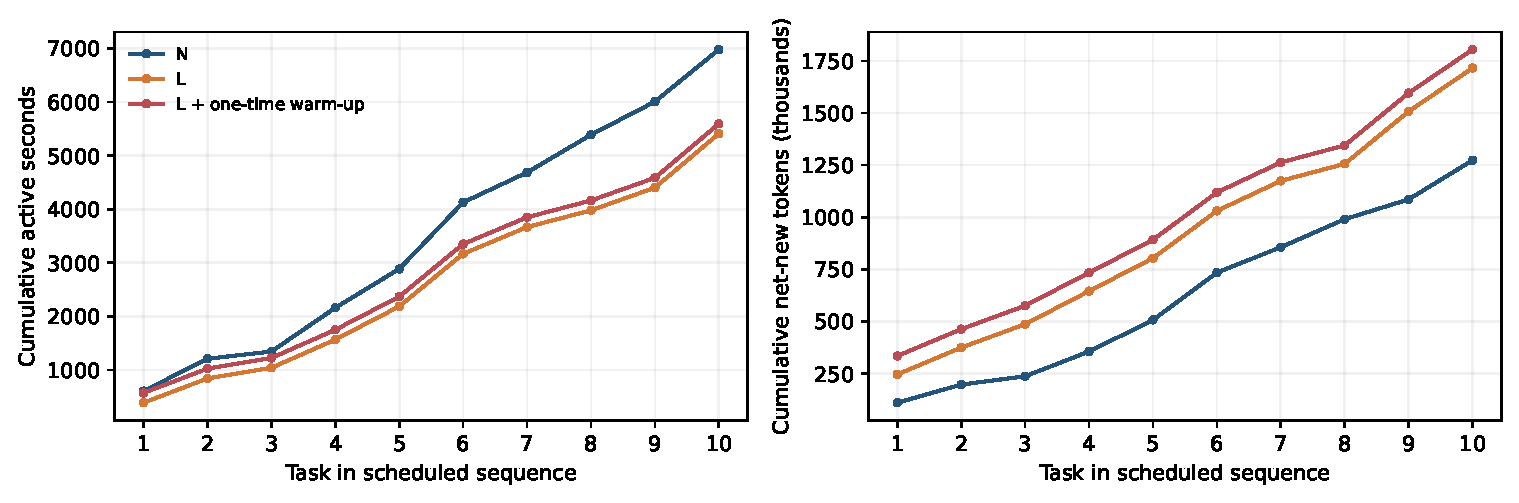
\includegraphics[width=.95\textwidth]{../benchmark/figures/12_cumulative_warm.pdf}
\caption{Cumulative contestant-active work in the ten-task order shown. The
red L curve charges the one-time scout once. This is not parallel campaign
makespan.\cite{summary,plotcode}}
\label{fig:cumulative}\end{figure}

\phaseoutfig{12a_cumulative_phase_time}{Running formalization and proof
seconds shown separately in scheduled task order. Panel titles give the
final cumulative L gain; the one-time scout is not assigned to either phase.}
\phaseoutfig{12b_cumulative_phase_tokens}{Running formalization and proof
net-new tokens shown separately in scheduled task order. Panel titles give
the final cumulative L gain; the one-time scout is not assigned to either phase.}

\clearpage
\section{Library usage and overlap}

The declaration scan uses elaborated constants in final L statements and
kernel-accepted proof terms, including proof-local helper bodies. It is not
an import or text-match count. Of the ten tasks, nine had
substantive NumStability statement reach, and all ten had direct proof-term
reach. Exact names, counts, and statement/proof surfaces are in the
machine-readable declaration ledger.\src{declscan,taskledger}

The primary measure is the number of \emph{distinct directly reached}
NumStability declarations in the accepted L artifact. It is applied to the
surface corresponding to each outcome: statement names for formalization,
proof-term names for proof, and their deduplicated union for total outcomes.
This is one counting rule, not three competing definitions of use. Other
source and dependency measures, including recursive statement dependencies
(RS and RF), remain secondary diagnostics in
Appendix~\ref{app:secondarymetrics}.
Imports alone are not counted by any measure. Literal source-text counts
of \texttt{NumStability.*} are excluded: they cannot resolve unqualified
uses brought into scope by \texttt{open NumStability}. We therefore also
recompiled the hash-frozen accepted L source files offline to obtain Lean's
namespace-resolved source-reference index. Its count of written references,
including repeated uses of a name, is shown in
Table~\ref{tab:sourcereferences}. The earlier literal-text diagnostics
remain in Appendix~\ref{app:secondarymetrics}.
\src{usagepoints,declscan,metriccode,sourcerefs}

The phase-specific versions of this one direct-use measure are:
\begin{itemize}\setlength{\itemsep}{1pt}
\item \emph{Direct statement (DS):} distinct NumStability constants found
  by Lean in the accepted target type and statement-local definitions.
\item \emph{Direct proof (DP):} distinct NumStability constants found in
  the accepted proof term and proof-local helper bodies.
\item \emph{Direct union (DU):} distinct names in DS $\cup$ DP; a name
  appearing on both surfaces is counted once.
\end{itemize}

Here \emph{distinct} means unique fully resolved Lean declaration names:
using the same NumStability lemma several times in one accepted artifact
still contributes one to that artifact's count. DP is the natural
library-use count for a proof-only comparison. In these ten tasks DP and
DU happen to have identical values, while DS is used for the separate
formalization-phase comparison.

For example, RUMP12-THM3.4 opens the NumStability namespace and uses its
declarations without writing the prefix: its literal qualified-source count
is zero, while Lean finds 39 distinct proof-term declarations. This is why
the source-text counts are not treated as measures of library use here.
The reported coefficients use unrounded gains and average ranks for tied counts.
\src{usagepoints,declscan,phasepoints,metriccode,evidence}

The direct elaborated-name scan permits a phase split. We compare
statement names with formalization outcomes, proof-term names with proof
outcomes, and their deduplicated union with total outcomes. Formalization
and proof code-size outcomes use statement and proof lines respectively;
total code size is their sum. Time and net-new-token gains use the same
phase boundaries. The one-time scout is excluded from all three views.
\src{phasepoints,usagepoints,taskledger}

\begin{table}[H]\centering\small
\begin{tabular}{@{}lrrr@{}}\toprule
Use surface / measured phase & Time $\rho$ & Tokens $\rho$ & Code lines $\rho$\\\midrule
Formalization / Statement declarations & -0.12 & -0.31 & +0.79 \\
Proof / Proof-term declarations & +0.56 & +0.50 & +0.64 \\
Total / Statement/proof union declarations & +0.56 & +0.54 & +0.72 \\
\bottomrule

\end{tabular}
\caption{Phase-aligned Spearman correlations for all ten pairs. The
statement-use count correlates with shorter statement code but not with
faster or lower-token formalization in this sample. These descriptive
rank associations do not establish that using a declaration caused a gain.
\cite{phasepoints,metriccode}}
\label{tab:phasecorrelations}
\end{table}

In this corpus every direct statement name also occurs in the proof-term
name set; the union count consequently equals the proof count. That
identity is a property of these ten files, not a general equivalence of
statement and proof use. The machine-readable ledger also records
proof-exclusive names to reveal this overlap. The phase split makes the
main asymmetry visible: statement use has $\rho=-0.12$ with formalization
time and $-0.31$ with formalization tokens, whereas proof-term use has
$\rho=+0.56$ with proof time and $+0.64$ with proof lines.\src{phasepoints}

DU has $\rho=+0.56$ with total-time gain, $\rho=+0.72$ with combined
statement-plus-proof-line gain, and $\rho=+0.54$ with total net-new-token
gain. Since DU equals DP for every task here, this is the same declaration
count that correlates $+0.64$ with proof-line gain. Declaration count can also track problem
complexity, and with only ten outcome-aware selected tasks none of these
coefficients identifies a causal benefit. Model search appears in archived
events, but no causal ``query overhead'' variable was isolated.
\src{usagepoints,evidence}

\subsection{Phase-matched usage plots}

The following three figures each contain three gain panels: time,
net-new tokens, and accepted code lines. Thus all nine phase-by-outcome
comparisons are visible without repeating a full set of plots for each
surface. Positive N-to-L percentage gain favors L. Numbered dots match
Table~\ref{tab:usecounts}; slight horizontal offsets reveal tied counts,
but the printed Spearman coefficients use unoffset values. No trend line
or p-value was used to select the measure. For readability, every
horizontal axis says \emph{Library usage}. In the formalization figure
this means DS (distinct declarations in the accepted statement); in
the proof figure it means DP (distinct declarations in the proof term
and proof-local helpers); in the total figure it means DU (their
deduplicated union). These are counts, not a subjective score.
\src{phasepoints,metriccode}

\phasefig{19a_statement_use_formalization}{Library usage versus
formalization-time, formalization-token, and statement-line gains.
Here usage is DS: distinct direct NumStability names in the accepted
statement.}
\phasefig{19b_proof_use_proving}{Library usage versus proof-time,
proof-token, and kernel-accepted proof-line gains. Here usage is DP:
distinct direct NumStability names in the accepted proof term and
proof-local helpers.}
\phasefig{19c_union_use_total}{Library usage versus total active-time,
total net-new-token, and combined statement-plus-proof-line gains.
Here usage is DU: the distinct union of statement and proof names,
counting any shared name once.}

\clearpage
\subsection{Gain--gain diagnostics}

The two gain--gain plots remain separate diagnostics: formalization versus
proof time, and active time versus net-new tokens. Both axes are N-to-L
percentage gains; zero lines distinguish gains from losses. Their points
use the same task-number key and no reuse-score coloring.\src{usagepoints}

\metricfig{18b_formal_proof_gain}{Formalization-time gain versus proof-time gain.
The upper-right quadrant means L was faster in both stages.}{+0.27}
\metricfig{18a_time_token_gain}{Total active-time gain versus total net-new-token
gain. The upper-right quadrant means L was faster and used fewer net-new
tokens.}{+0.15}

\subsection{Submission counts and concrete examples}

\begin{figure}[H]\centering
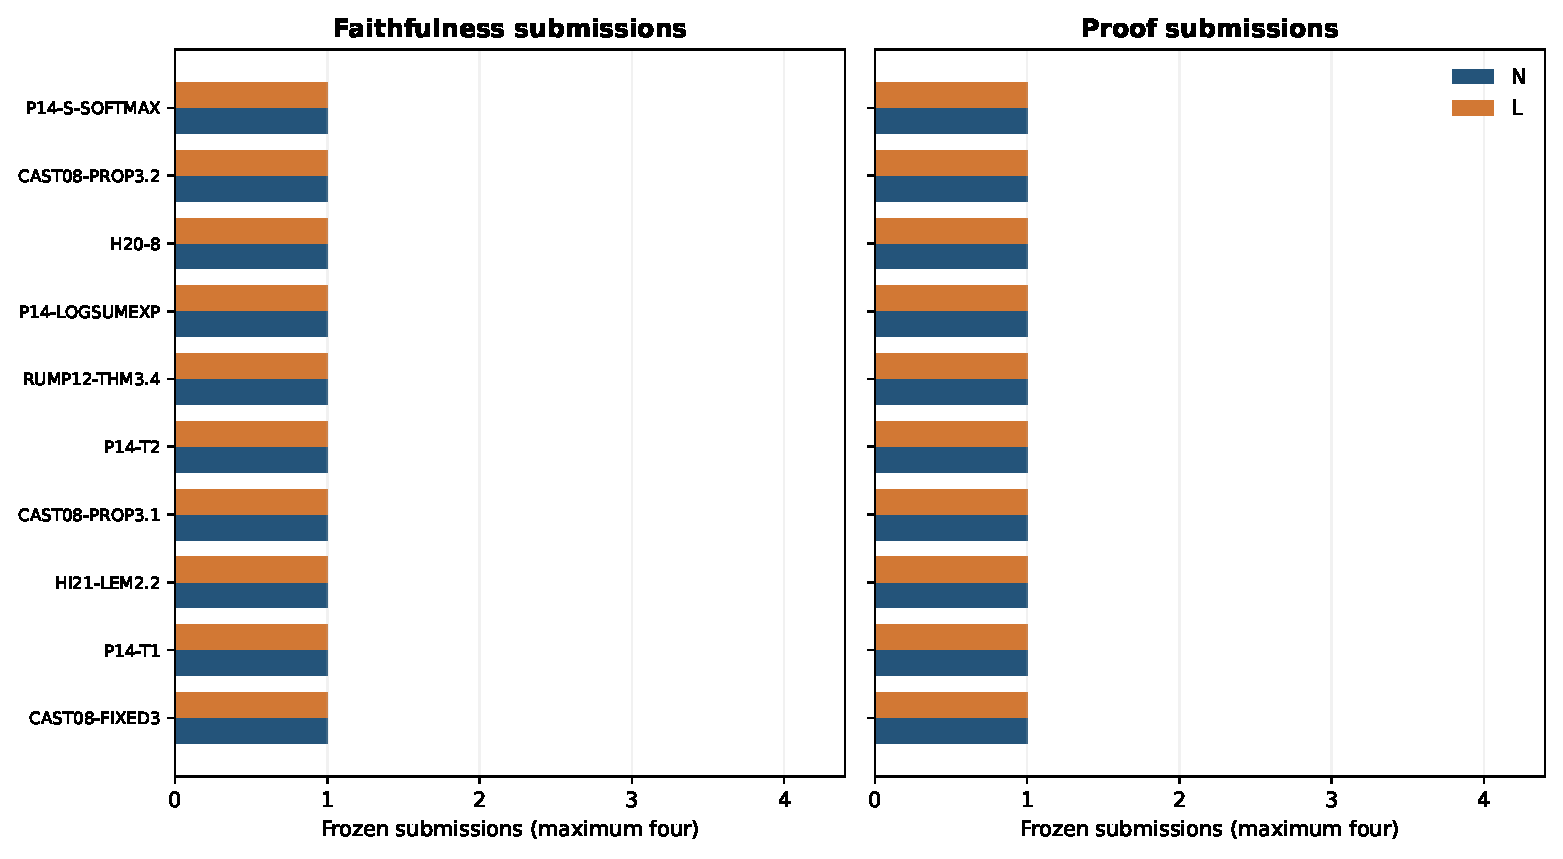
\includegraphics[width=.96\textwidth]{../benchmark/figures/16_attempts.pdf}
\caption{Frozen statement and proof submissions per task and condition.
Each stage allowed at most four submissions. Values come from the sealed
paired ledger.\cite{taskledger,plotcode}}
\end{figure}

Concrete examples show reusable material: CAST08-FIXED3 used dot-product
and recursive-sum interfaces, reducing proof code from 325 to 221 lines;
CAST08-PROP3.1 used summation/error declarations and reduced 373 to 200;
H20-8 used least-squares backward-error interfaces and reduced 243 to 167.
There are exceptions even with direct proof use: P14-LOGSUMEXP was faster but its L
proof had 257 versus 204 N lines. Usage counts record what was reached,
not what would have happened without the library.\src{taskledger,declscan}

\section{Conclusions and research direction}

The ten-task result is encouraging for NumStability's practical value. With
the library available, L produced faithful statements and complete proofs
for all ten tasks, used 19.7\% fewer nonblank proof-code lines, and spent
22.5\% less contestant-active time in aggregate. The gains arose mainly in
proving: L's proof stage was 29.9\% faster, whereas its formalization stage
was 7.3\% slower. L also used more net-new tokens overall. Thus the library
reduced elapsed work and proof code in this corpus, but did not improve every
measure.\src{summary,taskledger}

The token result is concentrated in the first phase, not spread evenly
across the workflow. L used 980,733 versus N's 399,748 net-new tokens to
reach faithful statements, an excess of 580,985. During proving, L used
734,899 versus 873,571, saving 138,672 tokens. Thus the formalization
excess more than accounts for the overall 442,313-token gap, while proof
reuse partly offsets it. In the archived per-condition usage records,
575,364 of L's formalization excess consists of additional \emph{uncached
input} tokens; only 5,621 consists of additional output tokens. The
measured difference is therefore input-heavy, not evidence that L wrote
much longer formalization responses. L's activity traces include library
inspection during this phase, but the records do not partition those
input tokens into search results, inherited orientation, prompts, and
other context. We therefore cannot attribute the gap specifically to
retrieval. The one-time scout's 88,468 net-new tokens are separate from
these task totals and would increase the token disadvantage if charged.
Conversely, L's lower proof-stage token use, proof time, and proof-code
size are consistent with useful declarations reducing work once a
faithful statement and applicable library interface are in place; this
phase comparison alone does not establish causation.
\src{summary,taskledger,evidence,metrics,warmscout}

The observed-use analysis points in a similarly positive, though not
absolute, direction. Across these ten tasks, greater direct proof-term use
was associated with larger proof-time and proof-line gains (Spearman
$\rho=+0.56$ and $+0.64$); combined statement/proof use was associated with
larger total-time and total-code gains ($\rho=+0.56$ and $+0.72$). These
positive trends support the interpretation that reusable declarations can
provide leverage when they fit the task. Individual exceptions remain, and
statement use did not show a positive formalization-time association in
this sample. Usage was observed after the agent worked, so these
correlations do not show that adding one more declaration would itself
cause a proportional gain.\src{phasepoints,usagepoints,taskledger}

A separate 30-task fixed-target HighamBench scope analysis supplies a useful
counterpoint: 17 of its 30 retained tasks had no NumStability dependency in
any of their three final L proofs. Tasks with consistent observed library
use had more favorable average time and source-line outcomes than those
with no observed use, but the use groups also followed different historical
campaigns. That study used fixed Lean targets, different models and
protocols, and a post-run scope restriction, so its outcomes cannot be
pooled with this formalize-and-prove experiment. The absence of final use
is consistent with uneven effective coverage; by itself it does not tell
whether a task lacked relevant mathematics, the agent failed to find it,
or an interface or representation mismatch prevented reuse.\src{scope30}

Taken together, the results justify further development rather than a
claim of universal advantage. Broadening the library's numerical-stability
results, improving discoverability, and adding representation bridges are
concrete ways to increase the range of tasks on which its components can
be applied. The positive association between observed reuse and gains makes
that direction promising, while the exceptions and higher token use show
what still needs improvement. A prospectively chosen evaluation under one
consistent protocol would be the next test of whether broader coverage
translates into reliable gains beyond this selected corpus. The L scout
models reusable task-neutral familiarity, not a fine-tuned model, and no
individual declaration's causal contribution is isolated here.
\src{summary,phasepoints,scope30,protocol}

\clearpage
\section{Reproducibility and source trail}

This private branch provides the report source, reproducible plotting and
table programs, the ten-task ledgers and figures, an execution description,
archived prompts, the warm-scout record, and paired run evidence. The
plotting scripts check ten exact task identities, pair outcomes,
source-packet hashes, metric sums, accepted proof-file hashes, and direct
declaration names.
The repository verifier separately checks task directories and candidate
hashes. Source papers, the original campaign controller and journals,
authenticated Codex state, and compiled caches are not repackaged. The
source registry gives paper-PDF hashes and task-packet identities. This
archive supports inspection and figure regeneration, not a standalone
bit-for-bit rerun of the model campaign.\src{readme,summary,registry,evidence}

Install the report's pinned Python requirements, run
\path{Documentation/make_figures.py} and
\path{Documentation/make_phase_cumulative_figures.py} and
\path{Documentation/make_usage_metric_plots.py}, then compile this
\texttt{report.tex} using \texttt{latexmk}. All displayed aggregate rows
and task-level appendices are generated from the archived ten-task ledger;
figures use unrounded values. The phase script generates the running-gain
checkpoints in Table~\ref{tab:aggregate} and the six new phase figures.
The measured evidence is read-only: changing
any task, prompt, or library snapshot would require a new benchmark identity
rather than an edit to these results.\src{plotcode,phaseplotcode,readme,taskledger}

\clearpage
\appendix
\begin{center}
{\Large\bfseries Appendices}
\end{center}
\medskip
\section{Task-level numeric ledger}

The tables below list the ten tasks in their scheduled order. Formalization and proof times are contestant-active seconds; token
totals are net-new thousands. SS means substantive statement-declaration
count and PT means direct proof-term declaration count. AF/AP are L
formalization/proof submission counts. All exact-precision values and both
conditions' attempt counts are in the machine-readable ledger.
\src{taskledger,plotcode}

\begin{table}[htbp]\centering
\resizebox{\textwidth}{!}{\begin{tabular}{@{}lrrrrrrrr@{}}\toprule
Task & F-N & F-L & P-N & P-L & Total-N & Total-L & Tok-N(k) & Tok-L(k)\\\midrule
CAST08-FIXED3 & 123 & 112 & 481 & 275 & 603 & 387 & 111 & 246 \\
P14-T1 & 176 & 171 & 428 & 282 & 604 & 453 & 87 & 129 \\
HI21-LEM2.2 & 106 & 161 & 29 & 37 & 135 & 199 & 40 & 112 \\
CAST08-PROP3.1 & 170 & 180 & 646 & 347 & 816 & 527 & 119 & 159 \\
P14-T2 & 135 & 135 & 590 & 485 & 725 & 619 & 151 & 158 \\
RUMP12-THM3.4 & 156 & 230 & 1087 & 752 & 1243 & 982 & 227 & 227 \\
P14-LOGSUMEXP & 130 & 93 & 428 & 407 & 558 & 499 & 122 & 144 \\
H20-8 & 91 & 102 & 612 & 211 & 703 & 313 & 134 & 82 \\
CAST08-PROP3.2 & 155 & 124 & 464 & 300 & 619 & 423 & 95 & 251 \\
P14-SHIFTED-SOFTMAX & 148 & 183 & 823 & 826 & 972 & 1009 & 188 & 208 \\

\end{tabular}}
\caption{Task-level time and net-new token comparison, excluding warm-up.
\cite{taskledger,plotcode}}\label{tab:times}
\end{table}
\begin{table}[htbp]\centering
\resizebox{\textwidth}{!}{\begin{tabular}{@{}llrrrrrrrr@{}}\toprule
Task & Cluster & Stmt-N & Stmt-L & Proof-N & Proof-L & SS & PT & AF & AP\\\midrule
CAST08-FIXED3 & CAST08 & 44 & 39 & 325 & 221 & 2 & 9 & 1 & 1 \\
P14-T1 & P14 & 27 & 29 & 201 & 227 & 2 & 7 & 1 & 1 \\
HI21-LEM2.2 & HI21 & 26 & 36 & 39 & 49 & 4 & 4 & 1 & 1 \\
CAST08-PROP3.1 & CAST08 & 40 & 39 & 373 & 200 & 1 & 9 & 1 & 1 \\
P14-T2 & P14 & 35 & 37 & 364 & 345 & 0 & 13 & 1 & 1 \\
RUMP12-THM3.4 & RUMP12 & 31 & 27 & 599 & 333 & 7 & 39 & 1 & 1 \\
P14-LOGSUMEXP & P14 & 28 & 27 & 204 & 257 & 2 & 8 & 1 & 1 \\
H20-8 & H20 & 25 & 20 & 243 & 167 & 5 & 26 & 1 & 1 \\
CAST08-PROP3.2 & CAST08 & 37 & 36 & 329 & 245 & 2 & 11 & 1 & 1 \\
P14-SHIFTED-SOFTMAX & P14 & 40 & 47 & 481 & 493 & 1 & 3 & 1 & 1 \\

\end{tabular}}
\caption{Final code size, declaration reach, and L submission counts.
\cite{taskledger,declscan,plotcode}}\label{tab:code}
\end{table}

\clearpage
\section{Observed-use count ledger}

DS and DP are distinct direct statement and proof declarations; DU is their
deduplicated union. The proof-exclusive column makes their relationship
visible. The numbered task key matches every usage--gain
figure. Full accepted proof paths, hashes, exact gains, and unrounded
correlations are in the metric ledger.\src{usagepoints,metriccode}

\begin{table}[htbp]\centering
\begin{tabular}{@{}rlrrrr@{}}\toprule
\# & Task & DS & DP & DP$\setminus$DS & DU\\\midrule
1 & CAST08-FIXED3 & 5 & 9 & 4 & 9  \\
2 & P14-T1 & 3 & 7 & 4 & 7  \\
3 & HI21-LEM2.2 & 4 & 4 & 0 & 4  \\
4 & CAST08-PROP3.1 & 4 & 9 & 5 & 9  \\
5 & P14-T2 & 0 & 13 & 13 & 13  \\
6 & RUMP12-THM3.4 & 8 & 39 & 31 & 39  \\
7 & P14-LOGSUMEXP & 3 & 8 & 5 & 8  \\
8 & H20-8 & 5 & 26 & 21 & 26  \\
9 & CAST08-PROP3.2 & 5 & 11 & 6 & 11  \\
10 & P14-SHIFTED-SOFTMAX & 1 & 3 & 2 & 3  \\
\bottomrule

\end{tabular}
\caption{One direct-use count applied to the statement (DS), proof term
(DP), and their union (DU). All ten DS sets are subsets of DP, so DU=DP
in this corpus.\cite{phasepoints,metriccode}}\label{tab:usecounts}
\end{table}

\subsection{Cross-phase direct-use diagnostics}

For completeness, the archived plots below compare statement and proof
declaration counts against the same three \emph{overall} outcomes. They are
not phase-matched and are therefore excluded from the main comparison.
The DU version duplicates the DP counts exactly for these ten tasks; its
underlying plot remains in the evidence bundle but is not reproduced here.
\src{usagepoints,phasepoints,metriccode}

\usagefig{17c_direct_statement}{Statement declarations (DS) versus overall
time, proof-line, and token gains. Statement reach does not itself show
which proof lemmas were reused.}
\usagefig{17d_direct_proof}{Proof-term declarations (DP) versus overall
time, proof-line, and token gains. DP has the same task counts as DU here,
but proof LOC is a different outcome from total LOC.}

\subsection{Repeated uses written in Lean source}

DS, DP, and DU deduplicate declaration names. To measure how often the
agent \emph{wrote a reference} to a library declaration, we use Lean's
\texttt{.ilean} source-reference index from each hash-verified accepted L
\texttt{Candidate.lean}. This resolves opened namespaces, excludes imports
and comments, and counts repeated citations separately. It includes helper
declarations in the file, so its distinct-source column is not necessarily
identical to DU, which is based on the target's elaborated statement and
proof closure. Conversely, automatically inserted or tactic-selected
constants can occur in elaborated proof terms without a written citation.
This metric measures explicit source-level reuse, not all semantic proof
dependencies.\cite{sourcerefs,sourcecode}

\begin{table}[H]\centering\small
\begin{tabular}{@{}rlrr@{}}\toprule
\# & Task & Distinct source names & Written references\\\midrule
1 & CAST08-FIXED3 & 9 & 34 \\
2 & P14-T1 & 7 & 81 \\
3 & HI21-LEM2.2 & 4 & 16 \\
4 & CAST08-PROP3.1 & 8 & 48 \\
5 & P14-T2 & 13 & 55 \\
6 & RUMP12-THM3.4 & 32 & 94 \\
7 & P14-LOGSUMEXP & 7 & 74 \\
8 & H20-8 & 25 & 87 \\
9 & CAST08-PROP3.2 & 11 & 45 \\
10 & P14-SHIFTED-SOFTMAX & 3 & 11 \\
\bottomrule

\end{tabular}
\caption{Namespace-resolved NumStability source citations in each final
accepted L file. For P14-T2, 13 distinct names were cited 55 times;
repeated citations are included in the latter count.\cite{sourcerefs}}
\label{tab:sourcereferences}
\end{table}

\begin{table}[H]\centering\small
\begin{tabular}{@{}lrrr@{}}\toprule
Source-level use & Time $\rho$ & Proof LOC $\rho$ & Net-new tokens $\rho$\\\midrule
Distinct source names & +0.58 & +0.64 & +0.52 \\
Written source references & +0.36 & +0.21 & +0.61 \\
\bottomrule

\end{tabular}
\caption{Descriptive Spearman correlations of distinct and repeated
source references with total active-time, proof-line, and total net-new-token
gains. These cross-task associations are not causal.\cite{sourcerefs,sourcestats}}
\label{tab:sourcecorrelations}
\end{table}

\begin{figure}[H]\centering
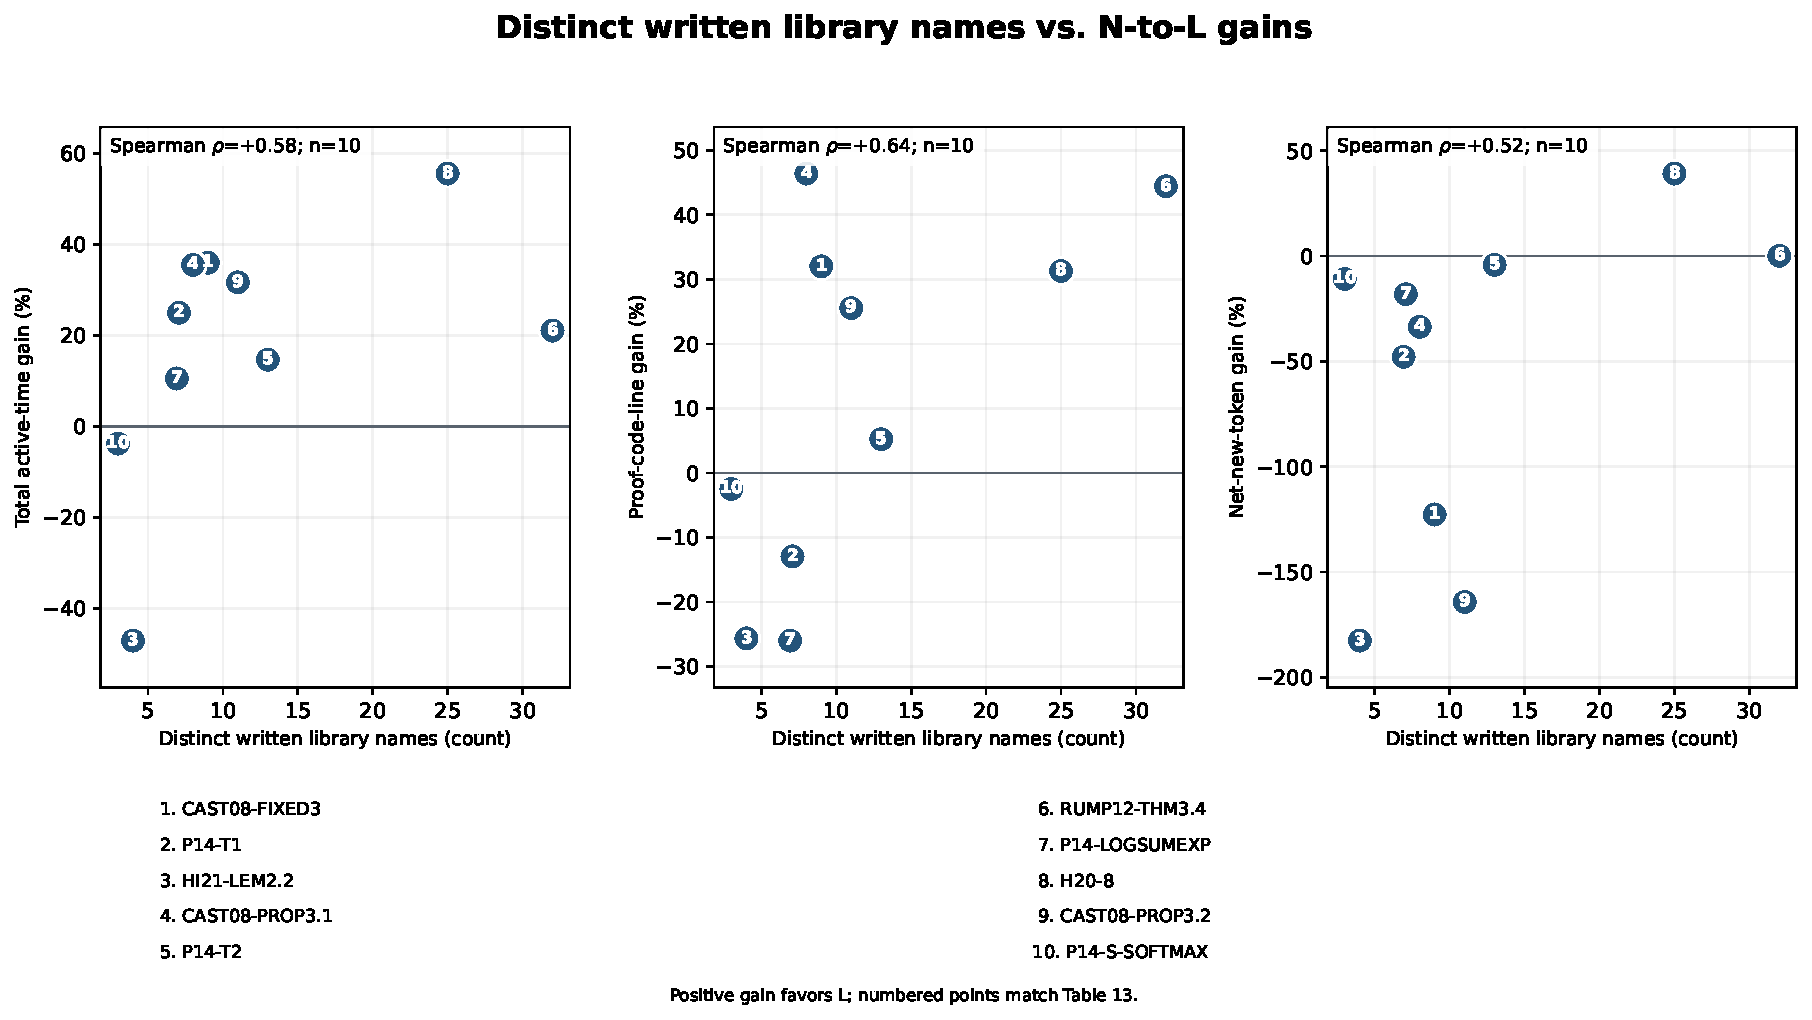
\includegraphics[width=\textwidth]{../benchmark/figures/20a_source_distinct_gains.pdf}
\caption{Distinct NumStability names cited in the accepted Lean source versus
total active-time, proof-code-line, and net-new-token gains. Numbered
points match Table~\ref{tab:sourcereferences}; positive gain favors L.
Each panel shows its descriptive Spearman coefficient ($n=10$).
\cite{sourcerefs,sourcestats,sourcefigcode}}
\label{fig:sourcedistinct}
\end{figure}

\begin{figure}[H]\centering
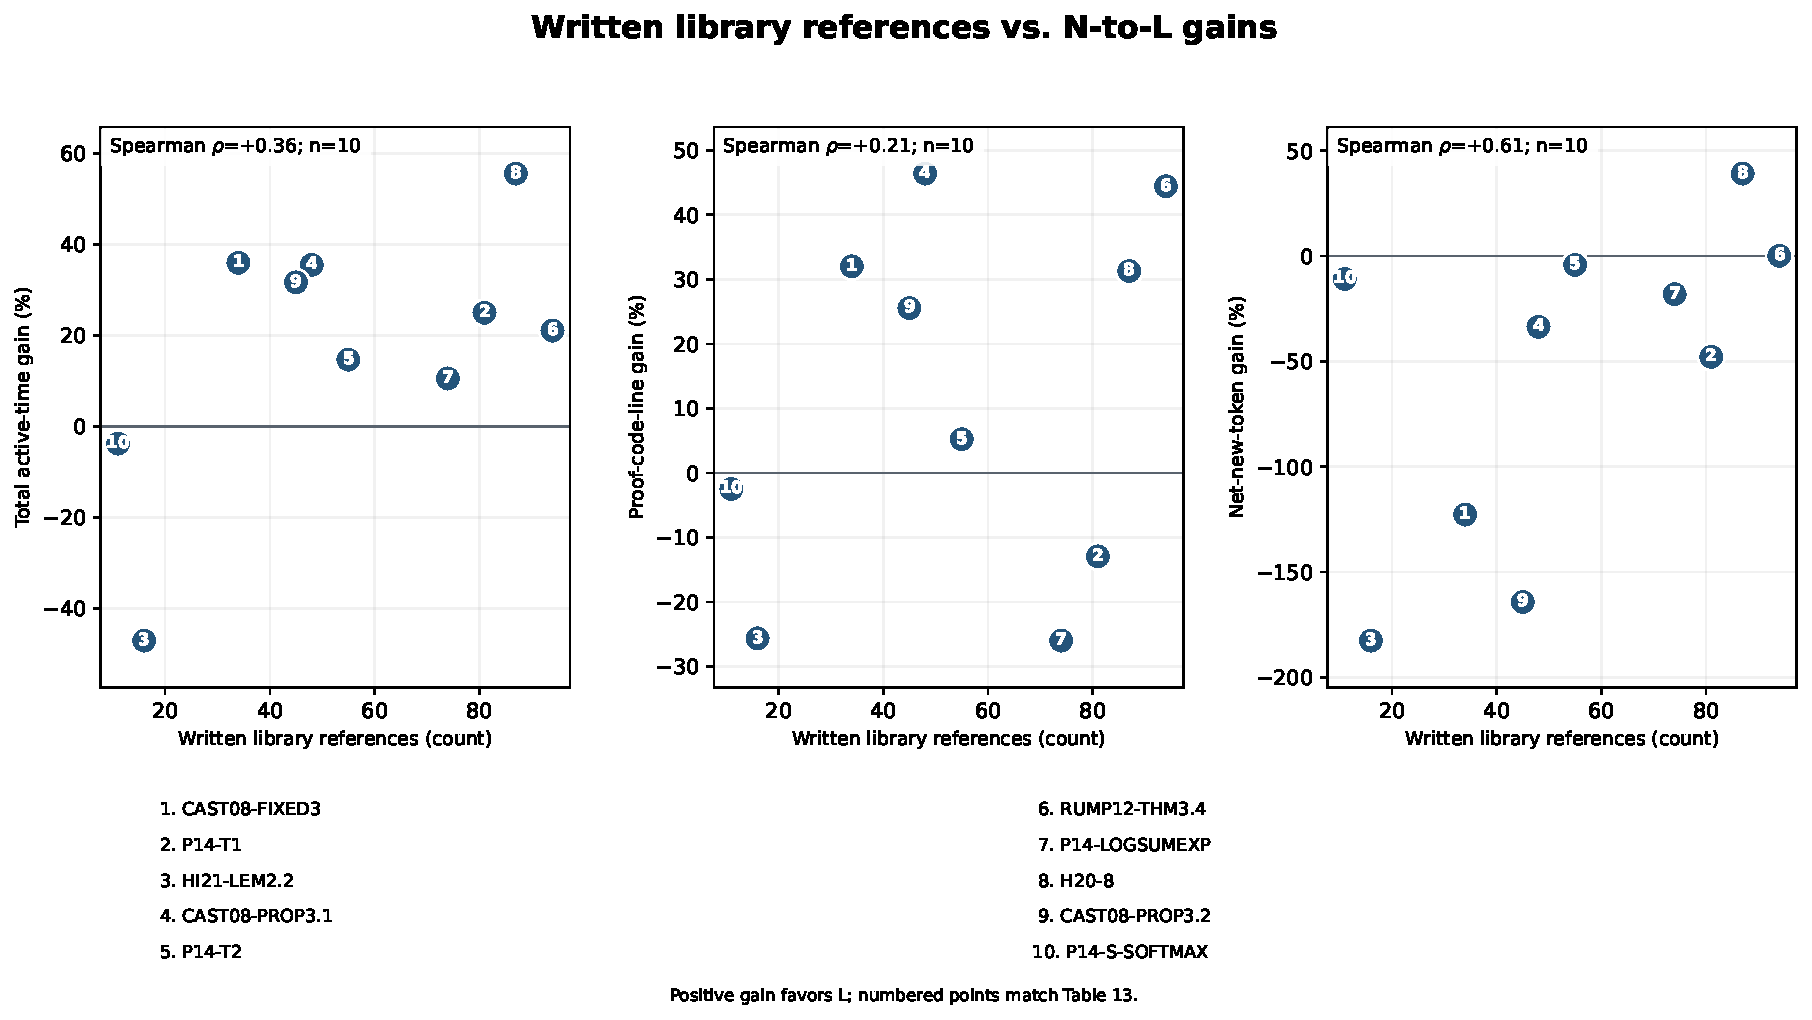
\includegraphics[width=\textwidth]{../benchmark/figures/20b_source_references_gains.pdf}
\caption{The same paired gains against all written NumStability references,
including repeated citations of the same name. This count is
namespace-resolved but covers the complete accepted L file, not the proof
phase alone. Numbered points match Table~\ref{tab:sourcereferences};
positive gain favors L.\cite{sourcerefs,sourcestats,sourcefigcode}}
\label{fig:sourcerepeats}
\end{figure}

\clearpage
\section{Direct declaration-usage index}

Family labels are descriptive; the JSON declaration scan contains exact
elaborated names in statements and proof terms. Imports and text-only
mentions are not counted.\src{declscan,taskledger}

\small
\begin{longtable}{@{}p{.22\textwidth}p{.27\textwidth}rp{.3\textwidth}r@{}}
\caption{Substantive statement and direct proof-term declaration families.
\cite{declscan,plotcode}}\\
\toprule Task & Statement family & $n$ & Proof family & $n$\\\midrule\endfirsthead
\toprule Task & Statement family & $n$ & Proof family & $n$\\\midrule\endhead
CAST08-FIXED3 & recursive sum, dot product & 2 & recursive sum, dot product, gamma bound & 9 \\
P14-T1 & recursive sum & 2 & recursive sum & 7 \\
HI21-LEM2.2 & sum tree & 4 & sum tree & 4 \\
CAST08-PROP3.1 & recursive sum & 1 & recursive sum, gamma bound & 9 \\
P14-T2 & none & 0 & gamma bound, product error & 13 \\
RUMP12-THM3.4 & finite FP format & 7 & finite FP format & 39 \\
P14-LOGSUMEXP & recursive sum & 2 & recursive sum, gamma bound & 8 \\
H20-8 & least squares & 5 & least squares & 26 \\
CAST08-PROP3.2 & recursive sum & 2 & recursive sum, gamma bound & 11 \\
P14-SHIFTED-SOFTMAX & infinity norm & 1 & infinity norm & 3 \\

\end{longtable}
\normalsize

\clearpage
\section{Secondary source and dependency diagnostics}\label{app:secondarymetrics}

Four archived counts are retained for transparency but excluded from the
main direct-use comparison. Qd counts distinct literal
\texttt{NumStability.*} source names and Qo counts their repeated literal
occurrences outside imports, comments, and strings. Both miss unqualified
names resolved by \texttt{open NumStability}; they are not namespace-complete
source-use counts. RS counts NumStability dependencies recursively reachable
from the accepted statement dossier, including generated declarations. RF
applies a syntactic generated-name filter to RS. Neither RS nor RF traverses
the target proof, and RF is not a certified public-API count. For example,
HI21-LEM2.2 has DS=4, RS=11, and RF=5 because the recursive scan reaches
compiler-generated names such as \texttt{SumTree.eval.match\_1}.
\cite{usagepoints,metriccode,declscan}

\begin{table}[H]\centering\small
\begin{tabular}{@{}rlrrrr@{}}\toprule
\# & Task & Qd & Qo & RS & RF\\\midrule
1 & CAST08-FIXED3 & 0 & 0 & 11 & 9 \\
2 & P14-T1 & 0 & 0 & 5 & 5 \\
3 & HI21-LEM2.2 & 0 & 0 & 11 & 5 \\
4 & CAST08-PROP3.1 & 8 & 48 & 7 & 7 \\
5 & P14-T2 & 11 & 38 & 0 & 0 \\
6 & RUMP12-THM3.4 & 0 & 0 & 22 & 21 \\
7 & P14-LOGSUMEXP & 0 & 0 & 5 & 5 \\
8 & H20-8 & 0 & 0 & 12 & 12 \\
9 & CAST08-PROP3.2 & 0 & 0 & 8 & 8 \\
10 & P14-SHIFTED-SOFTMAX & 0 & 0 & 1 & 1 \\
\bottomrule

\end{tabular}
\caption{Archived source-spelling and statement-dependency diagnostics;
none measures direct proof reuse.\cite{usagepoints,metriccode}}
\label{tab:suppcounts}
\end{table}

\begin{table}[H]\centering\small
\begin{tabular}{@{}lrrr@{}}\toprule
Secondary metric & Time $\rho$ & Proof LOC $\rho$ & Net-new tokens $\rho$\\\midrule
Distinct qualified source names & +0.05 & +0.30 & +0.20 \\
Qualified source occurrences & +0.12 & +0.39 & +0.15 \\
Recursive statement dependencies & +0.41 & +0.47 & +0.02 \\
Recursive dependencies, filtered & +0.67 & +0.66 & +0.14 \\
\bottomrule

\end{tabular}
\caption{The archived secondary correlations, shown separately so they
cannot be mistaken for primary direct-use evidence.\cite{usagepoints,metriccode}}
\label{tab:suppcorrelations}
\end{table}

\suppfig{17a_qualified_distinct}{Distinct explicitly qualified source names
(Qd); unqualified namespace-open uses are missed.}
\suppfig{17b_qualified_occurrences}{Repeated explicitly qualified source
names (Qo); unlike the namespace-resolved source references in
Table~\ref{tab:sourcereferences}, this misses unqualified uses.}
\suppfig{17f_recursive_statement}{Raw recursive dependencies of the
statement dossier (RS), including compiler-generated names.}
\suppfig{17g_recursive_filtered}{The same statement dependencies after
heuristic generated-name filtering (RF).}

\clearpage
\section{Source registry and immutable identities}

Every figure and numerical table derives from the ten-task ledger and
summary. Method claims are linked to the archival execution description,
prompts, paired run records, hardware snapshots, or proof evidence.
\src{summary,taskledger,readme}

Unless marked as part of the report bundle, paths in this section and the
bibliography are relative to the
\href{https://github.com/AlexGeorgantzas/NumStability/tree/ten_task_benchmark}{private NumStability repository}, branch \path{ten_task_benchmark}.

\begin{longtable}{@{}p{.22\textwidth}>{\RaggedRight\arraybackslash}p{.7\textwidth}@{}}
\toprule Source & Path / identity\\\midrule\endfirsthead
\toprule Source & Path / identity\\\midrule\endhead
Ten-task ledger & \path{benchmark/results/source_task_ledger.json}; its metadata records the sealed-result SHA-256.\\
Source registry & \path{benchmark/results/source_registry.json}; task packets and paper-PDF hashes.\\
Warm scout & \path{benchmark/evidence/warm-root.json}; SHA-256 begins \texttt{3401426d25ee278c}.\\
Direct declarations & \path{benchmark/results/declaration_scan.json}; exact elaborated names.\\
Observed-use metrics & \path{benchmark/results/usage_metric_points.json}; seven archived measures, including two excluded source-text diagnostics, accepted proof/dossier hashes, exact gains and rank correlations.\\
Source-reference scan (report bundle) & \path{sources/01-current-ten-task-report/Documentation/source_reference_counts.json}; accepted-candidate hashes, per-name counts, and resolved source sites.\\
Source-reference figures (report bundle) & \path{sources/01-current-ten-task-report/Documentation/make_source_reference_figures.py}; plots from the verified source-reference and paired-gain ledgers.\\
Phase-aligned metrics & \path{benchmark/results/phase_usage_points.json}; statement, proof, proof-exclusive, union counts, phase gains, correlations and source hashes.\\
Aggregate metrics & \path{benchmark/results/summary.json}; ten-task sums.\\
Measured pair evidence & \path{benchmark/runs/}; each task has N/L condition records and a paired report.\\
Library build & \path{benchmark/evidence/library-build-record.json}; SHA-256 begins \texttt{6f4581380982e51f}.\\
Runtime snapshot & \path{benchmark/evidence/runtime-snapshot.json}; SHA-256 begins \texttt{9fac78511309a591}.\\
\bottomrule
\end{longtable}

\clearpage
\section{Frozen task-neutral prompts}\label{app:prompts}

The following text is included verbatim from the archived prompt files;
the SHA-256 prefixes in the main text identify those files. The common
statement prompt was shared by N and L. Only L received the treatment
appendix and the one-time scout. The proof-stage base and strict no-hole
instruction applied to both conditions. Task-specific source packets and
observed effective messages are in the paired run records rather than
repeated here.\src{prompts,proofprompt,evidence}

\subsection{Common statement prompt}
\VerbatimInput[fontsize=\footnotesize,breaklines=true,breakanywhere=true]{../benchmark/prompts/common.md}

\subsection{L treatment appendix}
\VerbatimInput[fontsize=\footnotesize,breaklines=true,breakanywhere=true]{../benchmark/prompts/library_appendix.md}

\subsection{One-time L scout prompt}
\VerbatimInput[fontsize=\footnotesize,breaklines=true,breakanywhere=true]{../benchmark/prompts/scout.md}

\subsection{Shared proof-stage base prompt}
\VerbatimInput[fontsize=\footnotesize,breaklines=true,breakanywhere=true]{../benchmark/prompts/prove.md}

\clearpage
\subsection{Shared strict no-hole proof instruction}
\VerbatimInput[fontsize=\footnotesize,breaklines=true,breakanywhere=true]{../benchmark/prompts/PROOF_PROMPT.md}

\begin{thebibliography}{99}\footnotesize\RaggedRight\setlength{\itemsep}{0pt}\setlength{\parskip}{0pt}
\bibitem{summary} Ten-task aggregate metrics, \path{benchmark/results/summary.json}.
\bibitem{taskledger} Sealed N/L task records, \path{benchmark/results/source_task_ledger.json}; underlying pair reports are in \path{benchmark/runs/}.
\bibitem{plotcode} Standalone ten-task figure/table program, \path{Documentation/make_figures.py}; inputs are only the private ten-task ledgers.
\bibitem{phaseplotcode} Phase-specific and cumulative figure/table program, \path{Documentation/make_phase_cumulative_figures.py}; inputs are the archived paired ledger and summary.
\bibitem{registry} Task-packet and paper-source identities, \path{benchmark/results/source_registry.json}.
\bibitem{packets} Hash-frozen task packets, \path{benchmark/tasks/}; paper-PDF hashes are in the source registry.
\bibitem{protocol} Execution description, \path{benchmark/protocol/EXECUTION.md}; actual prompt hashes and outcomes are in the pair reports.
\bibitem{metrics} Metric definitions, \path{benchmark/protocol/METRICS.md}; exact values are in the ledgers.
\bibitem{prompts} Common statement prompt, treatment appendix, proof prompt, and scout prompt, \path{benchmark/prompts/}.
\bibitem{proofprompt} Strict zero-hole proof-stage instruction, \path{benchmark/prompts/PROOF_PROMPT.md}.
\bibitem{warmroot} Frozen task-neutral orientation record, \path{benchmark/evidence/warm-root.json}.
\bibitem{warmscout} Orientation prompt and observable transcript, \path{benchmark/evidence/warm-scout/}.
\bibitem{evidence} Archived paired prompts, candidates, effective audit prompts, validators, hardware, and final Lean files, \path{benchmark/runs/}.
\bibitem{buildrecord} NumStability full build record, \path{benchmark/evidence/library-build-record.json}.
\bibitem{librarysnapshot} Library snapshot metadata, \path{benchmark/evidence/library-snapshot.json}; source is in \path{NumStability/}.
\bibitem{runtimesnapshot} Runtime snapshot, \path{benchmark/evidence/runtime-snapshot.json}.
\bibitem{declscan} Direct elaborated declaration ledger, \path{benchmark/results/declaration_scan.json}.
\bibitem{usagepoints} Observed-use metric coordinates, accepted artifact hashes, and rank coefficients, \path{benchmark/results/usage_metric_points.json}.
\bibitem{phasepoints} Phase-aligned direct-use counts, gains, accepted artifact hashes, and rank coefficients, \path{benchmark/results/phase_usage_points.json}.
\bibitem{metriccode} Source/semantic scan and scatter-plot program, \path{Documentation/make_usage_metric_plots.py}.
\bibitem{sourcecode} Report-bundle hash-checking Lean source-reference extractor, \path{sources/01-current-ten-task-report/Documentation/make_source_references.py}.
\bibitem{sourcerefs} Report-bundle per-name, per-site namespace-resolved source-reference ledger, \path{sources/01-current-ten-task-report/Documentation/source_reference_counts.json}.
\bibitem{sourcestats} Report-bundle table generator and rank-correlation output, \path{sources/01-current-ten-task-report/Documentation/make_source_reference_tables.py} and \path{generated/source_reference_statistics.json}.
\bibitem{sourcefigcode} Report-bundle source-reference plotting code, \path{sources/01-current-ten-task-report/Documentation/make_source_reference_figures.py}; generated figures \path{benchmark/figures/20a_source_distinct_gains.pdf} and \path{benchmark/figures/20b_source_references_gains.pdf}.
\bibitem{scope30} Separate, post-run 30-task fixed-target scope analysis, \emph{NumStability Reuse in a 30-Task HighamBench Scope Analysis}, in this private repository's \path{tiered_benchmark_30} branch: \path{paper_bencmark/highambench/reports/full-report-scope30/report.tex}. Its task ledger is \path{paper_bencmark/highambench/reports/library-usage-analysis/task_usage.csv} on that branch. The companion study has a different protocol and is not part of this ten-task archive.
\bibitem{readme} Archive scope and rebuild instructions, \path{README.md} and \path{Documentation/README.md}.
\end{thebibliography}
\end{document}
